\documentclass[a4paper]{article}
\usepackage[T1]{fontenc}
\usepackage{fullpage}
\usepackage{graphicx}
\usepackage{url}

\usepackage{helvet}
\renewcommand{\familydefault}{\sfdefault}

%\usepackage[fontsize=18pt]{scrextend}
%\usepackage{setspace}
%\onehalfspacing

\title{Réalisation du «net code» d'un jeu vidéo simple\\ Présentation du projet}
\author{Projet de programmation système (R3.05)\\ Année 2022-2023}
\date{loig.jezequel@univ-nantes.fr}

\begin{document}
\maketitle{}

\section{Objectif du projet}

Le code d'un jeu vidéo très simple impliquant quatre personnages vous est fourni.
Dans la version actuelle de ce code, un personnage est contrôlé au clavier et les trois autres sont contrôlés par un générateur de nombres aléatoires.
Votre objectif sera de permettre que ces trois derniers personnages soient contrôlés par d'autres joueurs à travers le réseau.

\section{Description du jeu fourni}

Le jeu qui vous est fourni est un jeu de course à pied dans lequel il faut appuyer le plus vite possible sur la barre espace pour faire arriver son personnage le premier au bout du parcours.
Il se déroule en 5 étapes, qui sont décrites dans cette partie telles qu'elles fonctionnent actuellement.
Chacune de ces étapes devra être plus ou moins fortement modifiée au cours de ce projet pour permettre le jeu par le réseau.

Le code vous sera distribué en début de première séance.

Pour tester le jeu il suffit de récupérer ce code et (à condition d'avoir Go sur votre machine) d'utiliser \verb|go build| dans le répertoire où se trouve le fichier \verb|go.mod|.
Ceci construit un exécutable \verb|course| qui permet de lancer le jeu.

\subsection{Écran d'accueil}

Au lancement du jeu, un écran d'accueil s'affiche (figure~\ref{fig:titre}). Il suffit d'appuyer sur espace pour passer à l'étape suivante.

\begin{figure}[htbp]
  \centering
  
\includegraphics[width=400pt]{titre.png}
  \caption{Écran d'accueil}\label{fig:titre}
\end{figure}

\subsection{Choix des personnages}

La deuxième étape est la sélection de quatre personnages (figure~\ref{fig:selection}).
Le joueur peut sélectionner l'un d'entre eux (P0) à l'aide des flèches gauche et droite puis valider son choix avec la touche espace.
Les trois autres personnages sont sélectionnés au hasard.
Une fois les quatre personnages sélectionnés, le jeu passe à l'étape suivante.

\begin{figure}[htbp]
  \centering
  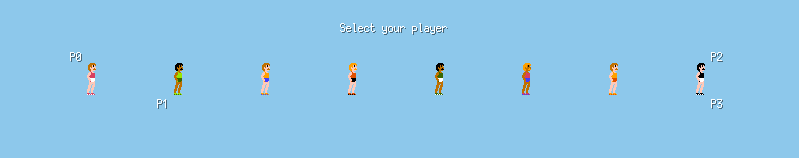
\includegraphics[width=400pt]{selection.png}
  \caption{Choix des personnages}\label{fig:selection}
\end{figure}

\subsection{Décompte}

La troisième étape est un décompte avant le début de la course.
Le joueur n'a rien à faire durant cette étape, on voit simplement 3, 2, 1 s'afficher à l'écran (figure~\ref{fig:decompte}).
Une fois le décompte terminé le jeu passe à l'étape suivante~: la course.

\begin{figure}[htbp]
  \centering
  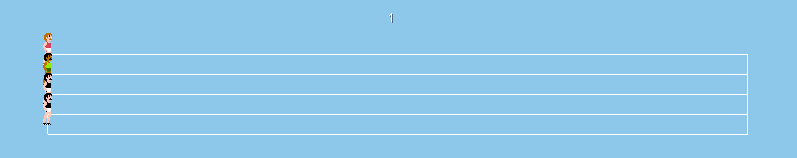
\includegraphics[width=400pt]{decompte.png}
  \caption{Décompte}\label{fig:decompte}
\end{figure}

\subsection{Course}

La quatrième étape est la course en elle même (figure~\ref{fig:course}).
Le joueur contrôle le personnage qu'il a préalablement sélectionné en appuyant le plus vite possible sur espace jusqu'à atteindre la ligne d'arrivée.
Les autres personnages sont contrôlés aléatoirement.
Une fois les quatre personnages arrivés, la course se termine et le jeu passe à l'étape suivante.

\begin{figure}[htbp]
  \centering
  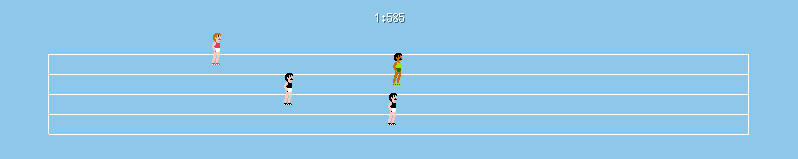
\includegraphics[width=400pt]{course.png}
  \caption{Course}\label{fig:course}
\end{figure}

\subsection{Résultats}

La dernière étape est celle des résultats.
Le temps de course de chacun des personnages est affiché, dans l'ordre de leur arrivée (figure~\ref{fig:resultats}).
Après cela, le joueur peut appuyer sur espace pour redémarrer une course (retour à l'étape du décompte).

\begin{figure}[htbp]
  \centering
  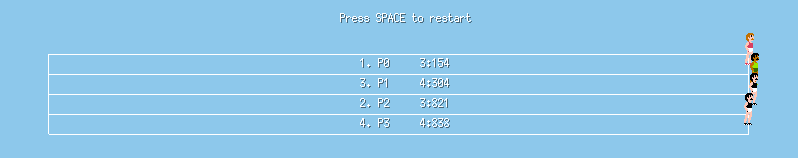
\includegraphics[width=400pt]{results.png}
  \caption{Résultats}\label{fig:resultats}
\end{figure}

\section{Description du jeu attendu}
\label{section:todo}

Il vous faudra modifier le code fourni afin de permettre à quatre joueurs de contrôler chacun un personnage du jeu et de jouer ensemble à travers le réseau.
Le principe sera que chaque joueur démarre le jeu sur sa machine (en indiquant l'adresse d'un serveur) et contrôle un personnage (le plus simple étant qu'il contrôle toujours P0) comme actuellement.
Par contre, au lieu d'être contrôlés aléatoirement, les trois autres personnages reflètent ce que font les trois autres joueurs sur leurs instances respectives du jeu.
Ceci implique que le jeu de chaque joueur retransmette à destination des autres jeux, via un serveur, des informations sur ce que fait le joueur.

\section{Ce que vous aurez à faire}

Pour obtenir la moyenne, il vous faut écrire un code Go qui réponde, au minimum, à la demande exprimée dans les différents sujets qui vous serons distribués au cours de ce projet.
Ce code reposera sur le code qui vous est fourni.

Pour nous faciliter la correction, il faudra identifier au mieux votre contribution~:
\begin{itemize}
  \item les nouvelles fonctions seront écrites dans des nouveaux fichiers,
  \item les modifications à mes fonctions seront clairement indiquées par des commentaires.
\end{itemize}
Votre code devra bien sûr être commenté pour indiquer l'utilité de chacune de vos fonctions (sur le modèle du code fourni) et, si besoin, décrire l'implémentation des plus complexes d'entre elles.

Pour obtenir une note supérieure à la moyenne il vous faudra ajouter des améliorations, parmi celles qui vous seront suggérées au cours du projet (plus vous en ajoutez, plus votre note sera élevée).

En plus du bon fonctionnement de votre programme, la qualité de votre code et de vos commentaires pourront bien sûr aussi améliorer ou réduire votre note. Du moment que le jeu tourne toujours de manière fluide (i.e. aux alentours de 60 frames par seconde) les performances de votre code ne seront par contre pas prises en compte de manière négative.

\section{Hypothèses simplificatrices}

Pour simplifier l'implémentation on considérera les hypothèses suivantes.

\begin{itemize}
\item Aucun joueur n'est déconnecté durant toute la durée du jeu.
\item Il y a un faible délai entre l'émission et la réception d'un message à travers le réseau.
\item Aucun message envoyé sur le réseau n'est perdu.
\item Les messages arrivent dans l'ordre où ils ont été émis (si m1 puis m2 sont envoyés par un programme p1 à destination d'un programme p2, alors p2 recevra toujours m1 avant m2).
\end{itemize}

\end{document}
